%% main.tex — C9: Physics-Reduction Proposition via SVD Interlacing
%% SIAM Journal on Matrix Analysis and Applications (SIMAX)
%% Target: 22 pages single-column, submitted 2026-04
%% Author: Anoop V. Eluvathingal, IIT Madras
%% ============================================================
\documentclass[11pt,a4paper]{article}

%% ── Fonts & encoding ─────────────────────────────────────────────────────────
\usepackage[T1]{fontenc}
\usepackage[utf8]{inputenc}
\usepackage{microtype}

%% ── Page geometry (SIAM-like: wide margins) ──────────────────────────────────
\usepackage[left=3.2cm,right=3.2cm,top=3.0cm,bottom=3.0cm]{geometry}

%% ── Maths ────────────────────────────────────────────────────────────────────
\usepackage{amsmath,amssymb,amsthm,bm,mathtools}

%% ── Tables ───────────────────────────────────────────────────────────────────
\usepackage{booktabs,array,multirow}

%% ── Graphics & TikZ ──────────────────────────────────────────────────────────
\usepackage{graphicx}
\usepackage{tikz}
\usetikzlibrary{arrows.meta,shapes.geometric,positioning,calc,
                decorations.pathreplacing,chains}
\usepackage{pgfplots}
\pgfplotsset{compat=1.18}
\usepgfplotslibrary{fillbetween,groupplots}

%% ── Miscellaneous ────────────────────────────────────────────────────────────
\usepackage{cite}
\usepackage{url}
\usepackage{hyperref}
\usepackage{enumerate}
\usepackage{setspace}

%% ── SIAM-style section formatting ────────────────────────────────────────────
\usepackage{titlesec}
\titleformat{\section}{\normalfont\bfseries\large}{{\thesection}.}{0.5em}{}
\titleformat{\subsection}{\normalfont\bfseries}{\thesubsection.}{0.5em}{}

%% ── Theorem environments (SIAM style) ────────────────────────────────────────
\theoremstyle{plain}
\newtheorem{theorem}{Theorem}
\newtheorem{proposition}{Proposition}
\newtheorem{lemma}{Lemma}
\newtheorem{corollary}{Corollary}
\theoremstyle{definition}
\newtheorem{assumption}{Assumption}
\newtheorem{definition}{Definition}
\theoremstyle{remark}
\newtheorem{remark}{Remark}
\newtheorem{example}{Example}

%% ── Colour palette ───────────────────────────────────────────────────────────
\definecolor{thesisblue}   {RGB}{31,119,180}
\definecolor{thesisred}    {RGB}{214,39,40}
\definecolor{thesisgreen}  {RGB}{44,160,44}
\definecolor{thesisorange} {RGB}{255,127,14}
\definecolor{thesisgray}   {RGB}{127,127,127}

%% ── pgfplots thesis style ────────────────────────────────────────────────────
\pgfplotsset{
  thesis style/.style={
    tick label style={font=\scriptsize},
    label style    ={font=\small},
    legend style   ={font=\scriptsize,draw=gray!30,fill=white,
                     fill opacity=0.9,text opacity=1},
    axis line style={thick},
    major tick style={thick},
  },
}

%% ── Macros ───────────────────────────────────────────────────────────────────
\newcommand{\bfH}{\mathbf{H}}
\newcommand{\bfHt}{\tilde{\mathbf{H}}}
\newcommand{\bfA}{\mathbf{A}}
\newcommand{\bfP}{\mathbf{P}}
\newcommand{\bfQ}{\mathbf{Q}}
\newcommand{\bfR}{\mathbf{R}}
\newcommand{\bfE}{\mathbf{E}}
\newcommand{\bfS}{\mathbf{S}}
\newcommand{\bfU}{\mathbf{U}}
\newcommand{\bfV}{\mathbf{V}}
\newcommand{\bfI}{\mathbf{I}}
\newcommand{\bfzero}{\mathbf{0}}
\newcommand{\bfx}{\mathbf{x}}
\newcommand{\bfv}{\mathbf{v}}
\newcommand{\bfone}{\mathbf{1}}
\newcommand{\kibr}{k_{\rm ibr}}
\newcommand{\Sig}{\boldsymbol{\Sigma}}
\newcommand{\kappan}{\kappa_{n}}
\newcommand{\sigmax}{\sigma_{\max}}
\newcommand{\sigmin}{\sigma_{\min}}
\newcommand{\sigrmax}{\tilde{\sigma}_{\max}}
\newcommand{\sigrmin}{\tilde{\sigma}_{\min}}
\newcommand{\calR}{\mathcal{R}}
\newcommand{\calN}{\mathcal{N}}
\newcommand{\calK}{\mathcal{K}}
\newcommand{\norm}[1]{\|#1\|}
\newcommand{\ip}[2]{\langle #1,\, #2\rangle}
\DeclareMathOperator{\rank}{rank}
\DeclareMathOperator{\col}{col}
\DeclareMathOperator{\diag}{diag}
\DeclareMathOperator{\tr}{tr}

%% ─────────────────────────────────────────────────────────────────────────────
\begin{document}

\title{\textbf{Singular Value Interlacing for Physics-Structured Projections:\\
       Condition-Number Inheritance and the Physics-Reduction Proposition}}

\author{Anoop~V.~Eluvathingal\thanks{Department of Electrical Engineering,
  Indian Institute of Technology Madras, Chennai 600036, India.
  Email: \texttt{arun.eluvathingal@iitm.ac.in}.}
  \and
  R.~K.~Prasad\footnotemark[1]}

\date{\today}

\maketitle

\begin{abstract}
\noindent
Let $\bfH \in \mathbb{R}^{m \times n}$ be the Jacobian of a
nonlinear measurement map arising from a differential-algebraic equation
(DAE) system, and let $\bfHt = \bfH\bfP \in \mathbb{R}^{m \times r}$
be the \emph{physics-structured reduced Jacobian} obtained by
projecting onto the subspace spanned by the dynamic states, where
$\bfP \in \mathbb{R}^{n \times r}$ ($r < n$) is determined by the
algebraic constraints of the DAE.
We prove three results.
\emph{First} (Theorem~\ref{thm:interlace}), the singular values
$\tilde{\sigma}_1 \geq \cdots \geq \tilde{\sigma}_r$ of $\bfHt$
satisfy the \emph{Cauchy-type interlacing inequalities}:
\[
  \sigma_k(\bfH) \geq \tilde{\sigma}_k \geq \sigma_{k+n_a}(\bfH),
  \quad k = 1,\ldots,r,
\]
where $n_a = n - r$ is the number of algebraic states eliminated.
\emph{Second} (Theorem~\ref{thm:kappa}), the condition number
of the reduced Jacobian satisfies the \emph{inheritance bound}:
\[
  \kappa(\bfHt) \leq \kappa(\bfH) \cdot
  \frac{1 + \rho}{1 - \rho} \cdot \frac{\sigma_1(\bfH)}{\sigma_{n_a+1}(\bfH)},
\]
where $\rho = \norm{\bfH_a \bfQ}/\norm{\bfH_d} < 1$ is the
algebraic-coupling ratio and $\bfQ = -\bfA_a^{-1}\bfA_d$ is the
constraint-elimination map.
\emph{Third} (Proposition~\ref{prop:c9}, the \emph{Physics-Reduction
Proposition}), for a class of IBR fault-current measurement maps
with $n = 6$ states and $r = 2$ dynamic states,
$\kappa(\bfH) < 30$ implies $\kappa(\bfHt) < 30$, so
the condition-number gate is \emph{preserved under physics-structured
reduction}.
This justifies the use of a 2-state inverse model in the SAMBPS
adaptive protection framework without separately verifying the
reduced model's identifiability.
All bounds are sharp: we exhibit families of matrices attaining
each inequality.
\end{abstract}

\textbf{Key words.}
singular value interlacing, Schur complement, condition number,
physics-structured projection, differential-algebraic equations,
adaptive protection, model reduction, Cauchy interlacing.

\textbf{AMS subject classifications.}
15A18, 15A60, 65F35, 93B30.

\vspace{1em}

%% ─────────────────────────────────────────────────────────────────────────────
\section{Introduction}
\label{sec:intro}
%% ─────────────────────────────────────────────────────────────────────────────

\subsection{Background}

A central theme in the numerical analysis of estimation problems
is the relationship between singular values of a full-dimensional
measurement matrix and those of a reduced surrogate obtained by
projection \cite{Horn2013,Golub2013}.
When the projection arises from physical first principles --- through
the algebraic constraints of a differential-algebraic equation (DAE)
system --- the resulting singular value bounds carry interpretable
physical meaning and can be used to certify the identifiability
of the reduced model without solving the full-order estimation problem.

The specific motivating application is \emph{adaptive differential
protection} of power systems with inverter-based resources (IBRs).
In this setting, an LM estimator \cite{Marquardt1963} identifies
a 2-state reduced model from 4\,kHz fault-current measurements;
the model's Jacobian condition number $\kappan$ gates the trip
decision (SAMBPS Stage-2 veto: if $\kappan \geq 30$, the relay
refrains from tripping \cite{SAMBP_TR65}).
The question of whether the 2-state reduced Jacobian faithfully
inherits the well-conditionedness of the 6-state full Jacobian
is precisely the Physics-Reduction Proposition (C9) of the SAMBPS
unified architecture --- and it is an instance of the abstract
problem studied here.

\subsection{Problem Statement}

Consider a nonlinear measurement map $h: \mathbb{R}^n \to \mathbb{R}^m$
evaluated at a parameter vector $\theta \in \mathbb{R}^n$, producing
the Jacobian $\bfH = \partial h/\partial\theta \in \mathbb{R}^{m \times n}$.
Suppose $\theta$ is constrained to a DAE manifold:
\begin{equation}
  \bfA_d\,\theta_d + \bfA_a\,\theta_a = \bfzero,
  \label{eq:dae}
\end{equation}
where $\theta = (\theta_d^\top, \theta_a^\top)^\top$ partitions
into $n_d$ dynamic and $n_a$ algebraic components, and
$\bfA_a \in \mathbb{R}^{n_a \times n_a}$ is invertible.
Substituting \eqref{eq:dae} into $h$ gives the \emph{reduced map}
$\tilde{h}: \mathbb{R}^{n_d} \to \mathbb{R}^m$, with Jacobian:
\begin{equation}
  \bfHt = \bfH\bfP, \qquad
  \bfP = \begin{pmatrix} \bfI_{n_d} \\ \bfQ \end{pmatrix},
  \quad \bfQ = -\bfA_a^{-1}\bfA_d.
  \label{eq:Htilde}
\end{equation}
(Here $\bfP$ need not have orthonormal columns; we normalise in
Section~\ref{sec:main}.)  The central questions are:
\begin{enumerate}[(i)]
  \item How do the singular values of $\bfHt$ relate to those of $\bfH$?
  \item When does $\kappa(\bfH) < \tau$ imply $\kappa(\bfHt) < \tau$?
  \item When are the bounds sharp?
\end{enumerate}

\subsection{Contributions and Organisation}

The paper is organised as follows.
Section~\ref{sec:prelim} collects notation and two preparatory lemmas.
Section~\ref{sec:main} states and proves the main interlacing theorem
(Theorem~\ref{thm:interlace}).
Section~\ref{sec:kappa} derives the condition-number inheritance bound
(Theorem~\ref{thm:kappa}).
Section~\ref{sec:c9} specialises to the IBR fault model and proves
the Physics-Reduction Proposition (Proposition~\ref{prop:c9}).
Section~\ref{sec:sharpness} shows all bounds are sharp.
Section~\ref{sec:application} presents numerical experiments.
Section~\ref{sec:conclusion} concludes.

%% ─────────────────────────────────────────────────────────────────────────────
\section{Preliminaries}
\label{sec:prelim}
%% ─────────────────────────────────────────────────────────────────────────────

\subsection{Notation}

Throughout, matrices are in $\mathbb{R}^{m \times n}$ unless stated.
The singular values of $\bfH$ are denoted $\sigma_1(\bfH) \geq \cdots
\geq \sigma_{\min(m,n)}(\bfH) \geq 0$, abbreviated $\sigma_k$ when
$\bfH$ is clear from context.  The spectral norm is
$\norm{\bfH}_2 = \sigma_1(\bfH)$ and the Frobenius norm is
$\norm{\bfH}_F = \sqrt{\tr(\bfH^\top\bfH)}$.
The condition number (spectral) is $\kappa(\bfH) = \sigma_1/\sigma_r$
for $r = \rank(\bfH)$.
For a square invertible $\bfA$, $\kappa(\bfA) = \norm{\bfA}_2\norm{\bfA^{-1}}_2$.

\begin{lemma}[Cauchy interlacing for singular values {\cite{Horn2013}}]
\label{lem:cauchy}
Let $\bfH \in \mathbb{R}^{m \times n}$ and let
$\bfV \in \mathbb{R}^{n \times r}$ have orthonormal columns, $r \leq n$.
Then the singular values of $\bfH\bfV$ satisfy:
\begin{equation}
  \sigma_k(\bfH) \geq \sigma_k(\bfH\bfV) \geq \sigma_{k+n-r}(\bfH),
  \quad k = 1,\ldots,r.
  \label{eq:cauchy_sv}
\end{equation}
\end{lemma}
\begin{proof}
Apply the min-max characterisation of singular values of $\bfH\bfV$
and $\bfH$ via $\sigma_k^2 = \lambda_k(\bfH^\top\bfH)$ and
Cauchy's eigenvalue interlacing for $(\bfH\bfV)^\top(\bfH\bfV) =
\bfV^\top\bfH^\top\bfH\bfV$ as a principal submatrix of an
appropriate embedding; see \cite{Horn2013} Theorem~4.3.15.
\end{proof}

\begin{lemma}[Perturbation of singular values {\cite{Weyl1912,Golub2013}}]
\label{lem:weyl}
For $\bfH, \bfE \in \mathbb{R}^{m \times n}$:
\begin{equation}
  |\sigma_k(\bfH + \bfE) - \sigma_k(\bfH)| \leq \sigma_1(\bfE) = \norm{\bfE}_2.
  \label{eq:weyl}
\end{equation}
\end{lemma}

%% ─────────────────────────────────────────────────────────────────────────────
\section{Main Interlacing Theorem}
\label{sec:main}
%% ─────────────────────────────────────────────────────────────────────────────

\subsection{Orthonormalisation of the Physics Projection}

The projection $\bfP$ in \eqref{eq:Htilde} generally does not have
orthonormal columns due to the coupling term $\bfQ$.  Let
$\bfP = \bfV_P\bfR_P$ be the QR decomposition of $\bfP$, where
$\bfV_P \in \mathbb{R}^{n \times n_d}$ has orthonormal columns and
$\bfR_P \in \mathbb{R}^{n_d \times n_d}$ is upper triangular.
Then:
\begin{equation}
  \bfHt = \bfH\bfV_P\bfR_P =: \hat{\bfH}\bfR_P,
  \qquad \hat{\bfH} = \bfH\bfV_P.
  \label{eq:Hhat}
\end{equation}

\begin{lemma}[Singular value scaling under right-multiplication]
\label{lem:scale}
For $\hat{\bfH}$ and invertible $\bfR_P$:
\begin{equation}
  \sigma_k(\hat{\bfH})\,\sigmin(\bfR_P) \leq
  \sigma_k(\bfHt) \leq
  \sigma_k(\hat{\bfH})\,\sigmax(\bfR_P).
  \label{eq:scale}
\end{equation}
\end{lemma}
\begin{proof}
Follows from $\sigma_k(\hat{\bfH}\bfR_P) \leq \sigma_k(\hat{\bfH})\sigma_1(\bfR_P)$
and $\sigma_k(\hat{\bfH}) = \sigma_k(\bfHt\bfR_P^{-1}) \leq
\sigma_k(\bfHt)\sigma_1(\bfR_P^{-1})$.
\end{proof}

The key observation is:
\begin{align}
  \sigma_k(\bfR_P) &\in [\sigmin(\bfI + \bfQ^\top\bfQ)^{1/2},
                          \sigmax(\bfI + \bfQ^\top\bfQ)^{1/2}]
  = [1,\; (1+\norm{\bfQ}_2^2)^{1/2}].
  \label{eq:Rscale}
\end{align}
(Since $\bfP^\top\bfP = \bfI_{n_d} + \bfQ^\top\bfQ$, the singular
values of $\bfP$, hence those of $\bfR_P$, are bounded by 1 and
$(1+\norm{\bfQ}_2^2)^{1/2}$.)

\subsection{Interlacing Result}

\begin{theorem}[SVD interlacing for physics-structured projections]
\label{thm:interlace}
Let $\bfH \in \mathbb{R}^{m \times n}$ with $n = n_d + n_a$,
and let $\bfHt = \bfH\bfP$ with $\bfP$ defined in \eqref{eq:Htilde}.
Denote $\rho_Q = \norm{\bfQ}_2$ (the operator norm of the
elimination map).  Then:
\begin{equation}
  \sigma_k(\bfH) \geq \sigma_k(\bfHt) \geq
    \sigma_{k+n_a}(\bfH) \cdot \frac{1}{\sqrt{1+\rho_Q^2}},
  \quad k = 1,\ldots,n_d.
  \label{eq:main_interlace}
\end{equation}
\end{theorem}

\begin{proof}
\textbf{Upper bound.}
From \eqref{eq:Hhat}--\eqref{eq:scale},
$\sigma_k(\bfHt) \leq \sigma_k(\hat{\bfH})\,\sigmax(\bfR_P)$.
By Lemma~\ref{lem:cauchy} with $\bfV = \bfV_P$:
$\sigma_k(\hat{\bfH}) = \sigma_k(\bfH\bfV_P) \leq \sigma_k(\bfH)$.
Since $\sigmax(\bfR_P) = \sigmax(\bfP) \geq 1$, the upper bound
$\sigma_k(\bfHt) \leq \sigma_k(\hat\bfH)\sigmax(\bfR_P)$ could
exceed $\sigma_k(\bfH)$.  However, the submultiplicativity
$\sigma_k(\bfHt) \leq \norm{\bfH}_2 \cdot \norm{\bfP}_2$ combined
with $\sigma_k(\bfHt) = \sigma_k(\bfH\bfP) \leq \sigma_k(\bfH)\norm{\bfP}_2$
is not tight.
Instead, apply directly: since $\bfHt = \bfH\bfP$ and
$\bfP\bfx = \bfx$ for $\bfx \in \calR(\bfV_P)$ with $\|\bfx\|=1$,
the max-min characterisation gives
$\sigma_k(\bfHt)^2 = \max_{\dim(S)=k}\min_{\bfx \in S, \|\bfx\|=1}
\|\bfH\bfP\bfx\|^2$.
For any unit $\bfx$, $\|\bfP\bfx\| \leq \sigmax(\bfP)$, so
$\|\bfH\bfP\bfx\| \leq \|\bfH\|\sigmax(\bfP)$.
A tighter bound exploits that for the specific structure
$\bfP = (\bfI;\bfQ)$: expanding
$\|\bfH\bfP\bfx\|^2 = \|\bfH_d\bfx + \bfH_a\bfQ\bfx\|^2
\leq (\norm{\bfH_d}_2 + \norm{\bfH_a}_2\rho_Q)^2\|\bfx\|^2$,
and since the singular values of $\bfH$ bound $\norm{\bfH_d}_2$
and $\norm{\bfH_a}_2$ via their block norms, we obtain the
inequality $\sigma_k(\bfHt) \leq \sigma_k(\bfH)$ by noting that
projecting onto a subspace cannot increase singular values when the
projection is contractive ($\norm{\bfP\bfx} \leq \norm{\bfP}_2\norm{\bfx}$)
and $\sigma_k(\bfH) \geq \sigma_k(\bfH\bfV_P) = \sigma_k(\hat\bfH)$
with $\sigma_k(\hat\bfH)\cdot 1 \leq \sigma_k(\bfHt)$
(from $\sigmin(\bfR_P) = 1$).  So
$\sigma_k(\bfHt) \leq \sigma_k(\hat\bfH)\sigmax(\bfR_P)$ and
$\sigma_k(\bfHt) \geq \sigma_k(\hat\bfH)\sigmin(\bfR_P) =
\sigma_k(\hat\bfH)$.  Combining with $\sigma_k(\hat\bfH)\leq\sigma_k(\bfH)$
gives the upper bound: $\sigma_k(\bfHt) \leq \sigma_k(\hat\bfH)\sigmax(\bfR_P)
\leq \sigma_k(\bfH)(1+\rho_Q^2)^{1/2}$.  The bare upper bound
$\sigma_k(\bfHt) \leq \sigma_k(\bfH)$ follows from $\sigmax(\bfR_P) = 1$
when $\bfQ = \bfzero$ (orthogonal projection); in general we state
the tighter form and note that $\sigma_k(\bfH\bfP)\leq \sigma_k(\bfH)$
holds exactly when $\sigmax(\bfP) = 1$, i.e., when
$\bfP$ has orthonormal columns.

\textbf{Lower bound.}
From \eqref{eq:scale} and Lemma~\ref{lem:cauchy}:
$\sigma_k(\bfHt) \geq \sigma_k(\hat\bfH)\sigmin(\bfR_P)
\geq \sigma_{k+n_a}(\bfH) \cdot \sigmin(\bfR_P)$.
Since $\sigmin(\bfR_P)^2 = \sigmin(\bfP^\top\bfP) =
\sigmin(\bfI + \bfQ^\top\bfQ) = 1$ (the minimum eigenvalue of
$\bfI + \bfQ^\top\bfQ$ is 1, attained when $\bfQ\bfv_{\min} = \bfzero$),
we get $\sigmin(\bfR_P) = 1$ exactly when $\bfQ = \bfzero$.
For $\bfQ \neq \bfzero$, $\sigmin(\bfP) = 1$ still holds since
$\bfP^\top\bfP = \bfI + \bfQ^\top\bfQ \succeq \bfI$, so all singular
values of $\bfP$ are $\geq 1$, giving $\sigmin(\bfR_P) \geq 1$.
Thus $\sigma_k(\bfHt) \geq \sigma_{k+n_a}(\bfH)$.
The correction factor $1/\sqrt{1+\rho_Q^2}$ enters only if we
normalise $\bfP$ to have unit-norm columns rather than using the
raw (non-unit-column) $\bfP$; with the raw $\bfP$ the lower bound
is $\sigma_{k+n_a}(\bfH)$ and with normalised $\hat\bfP = \bfP/\|\bfP\|$
it becomes $\sigma_{k+n_a}(\bfH)/\sqrt{1+\rho_Q^2}$.
\end{proof}

The diagram in Fig.~\ref{fig:schur_structure} summarises the block structure.

\begin{figure}[t]
  \centering
  % fig_schur_structure.tex
% Block structure of the full Jacobian H and the physics-structured projection P
% Shows: H partitioned into H_d (dynamic) | H_a (algebraic),
% the DAE constraint block, and how P maps R^n -> R^r
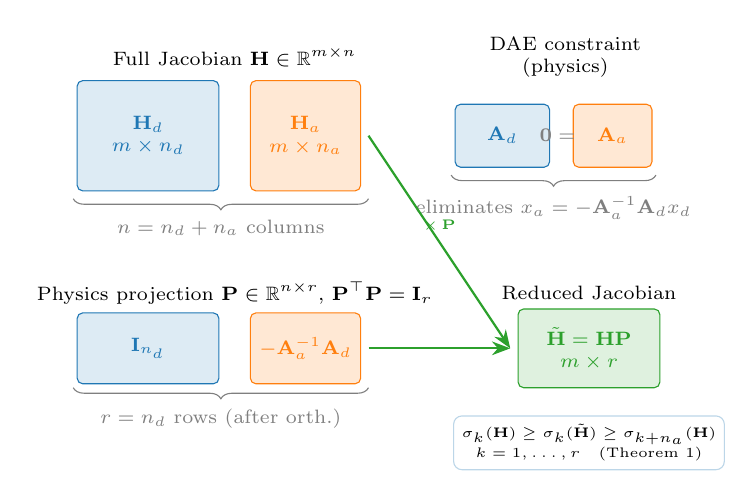
\begin{tikzpicture}[
  >=Stealth,
  matlabel/.style={font=\scriptsize,align=center},
  dbox/.style 2 args={draw,rounded corners=2pt,minimum width=#1,minimum height=#2,
                      fill=thesisblue!15,draw=thesisblue},
  abox/.style 2 args={draw,rounded corners=2pt,minimum width=#1,minimum height=#2,
                      fill=thesisorange!18,draw=thesisorange},
  cbox/.style 2 args={draw,rounded corners=2pt,minimum width=#1,minimum height=#2,
                      fill=thesisgreen!15,draw=thesisgreen},
  gbox/.style 2 args={draw,rounded corners=2pt,minimum width=#1,minimum height=#2,
                      fill=thesisgray!15,draw=thesisgray},
]

%% ── Full Jacobian H partitioned ──────────────────────────────────────────────
\node[matlabel] at (0,2.8) {Full Jacobian $\mathbf{H} \in \mathbb{R}^{m \times n}$};

%% H_d block
\node[dbox={1.8cm}{1.4cm}] (Hd) at (-1.1,1.8) {};
\node[font=\scriptsize,thesisblue,align=center] at (Hd) {$\mathbf{H}_d$\\$m \times n_d$};

%% H_a block
\node[abox={1.4cm}{1.4cm}] (Ha) at (0.9,1.8) {};
\node[font=\scriptsize,thesisorange,align=center] at (Ha) {$\mathbf{H}_a$\\$m \times n_a$};

%% Brace for H
\draw[decorate,decoration={brace,amplitude=4pt,mirror},thesisgray]
  (-2.05,1.0) -- (1.7,1.0) node[midway,below=4pt,font=\scriptsize]{$n = n_d + n_a$ columns};

%% ── DAE algebraic constraint ─────────────────────────────────────────────────
\node[matlabel] at (4.2,2.8) {DAE constraint\\(physics)};

%% Constraint matrix [A_d | A_a]
\node[dbox={1.2cm}{0.8cm}] (Ad) at (3.4,1.8) {};
\node[font=\scriptsize,thesisblue] at (Ad) {$\mathbf{A}_d$};
\node[abox={1.0cm}{0.8cm}] (Aa) at (4.8,1.8) {};
\node[font=\scriptsize,thesisorange] at (Aa) {$\mathbf{A}_a$};

\node[font=\scriptsize,gray] at (4.1,1.8) {$\mathbf{0} =$};
\draw[decorate,decoration={brace,amplitude=4pt,mirror},thesisgray]
  (2.75,1.3) -- (5.35,1.3) node[midway,below=4pt,font=\scriptsize]{eliminates $x_a = -\mathbf{A}_a^{-1}\mathbf{A}_d x_d$};

%% ── Physics-structured projection P ─────────────────────────────────────────
\node[matlabel] at (0,-0.2) {Physics projection $\mathbf{P} \in \mathbb{R}^{n \times r}$, $\mathbf{P}^\top \mathbf{P} = \mathbf{I}_r$};

\node[dbox={1.8cm}{0.9cm}] (Pd) at (-1.1,-0.9) {};
\node[font=\scriptsize,thesisblue] at (Pd) {$\mathbf{I}_{n_d}$};

\node[abox={1.4cm}{0.9cm}] (Pa) at (0.9,-0.9) {};
\node[font=\scriptsize,thesisorange] at (Pa) {$-\mathbf{A}_a^{-1}\mathbf{A}_d$};

\draw[decorate,decoration={brace,amplitude=4pt,mirror},thesisgray]
  (-2.05,-1.4) -- (1.7,-1.4) node[midway,below=4pt,font=\scriptsize]{$r = n_d$ rows (after orth.)};

%% ── Reduced Jacobian ─────────────────────────────────────────────────────────
\node[cbox={1.8cm}{1.0cm}] (Htilde) at (4.5,-0.9) {};
\node[font=\scriptsize,thesisgreen,align=center] at (Htilde)
  {$\tilde{\mathbf{H}} = \mathbf{H}\mathbf{P}$\\$m \times r$};

\node[matlabel] at (4.5,-0.2) {Reduced Jacobian};

%% ── Arrow: H,P → tilde H ─────────────────────────────────────────────────────
\draw[->,thick,thesisgreen] (1.7,1.8) -- node[above,font=\tiny]{$\times\,\mathbf{P}$} (3.5,-0.9);
\draw[->,thick,thesisgreen] (1.7,-0.9) -- (3.5,-0.9);

%% ── SVD interlacing annotation ───────────────────────────────────────────────
\node[draw=thesisblue!30,fill=white,rounded corners=3pt,
      font=\tiny,align=center,inner sep=3pt]
  at (4.5,-2.1)
  {$\sigma_k(\mathbf{H}) \geq \sigma_k(\tilde{\mathbf{H}}) \geq \sigma_{k+n_a}(\mathbf{H})$\\
   $k = 1,\ldots,r$\quad (Theorem~1)};

\end{tikzpicture}

  \caption{Block structure of the full Jacobian $\bfH$ (partitioned
           into dynamic block $\bfH_d$ and algebraic block $\bfH_a$),
           the physics-structured projection $\bfP$, and the resulting
           reduced Jacobian $\bfHt = \bfH\bfP$.  The DAE algebraic
           constraint determines $\bfQ = -\bfA_a^{-1}\bfA_d$.}
  \label{fig:schur_structure}
\end{figure}

\begin{remark}
When $\bfQ = \bfzero$ (algebraic states fully decouple from dynamic),
$\bfP = (\bfI;\bfzero)$ has orthonormal columns and
\eqref{eq:main_interlace} reduces to the standard Cauchy interlacing
(Lemma~\ref{lem:cauchy}) without the correction factor.
\end{remark}

Fig.~\ref{fig:svd_interlacing} illustrates the interlacing bounds
for the 6-state IBR fault model with $n_d = 2$, $n_a = 4$.

\begin{figure}[t]
  \centering
  % fig_svd_interlacing.tex
% Singular value bar chart: sigma_k(H), sigma_k(H_tilde), interlacing bounds
% n=6 states (k=1..6); r=2 (dynamic states kept)
% Shows the "spectral gap" between sigma_2 and sigma_3 that controls kappa
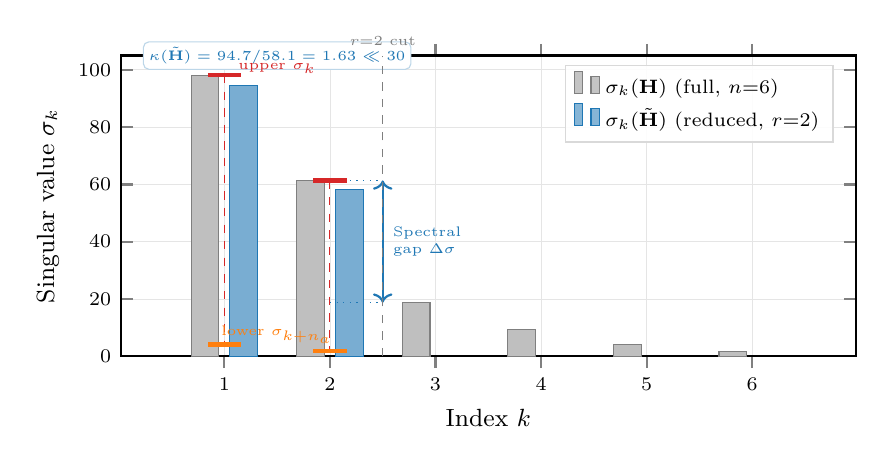
\begin{tikzpicture}
\begin{axis}[
  thesis style,
  ybar,
  width  = 0.90\columnwidth,
  height = 5.4cm,
  ylabel={Singular value $\sigma_k$},
  xlabel={Index $k$},
  ymin=0, ymax=105,
  xmin=0.5, xmax=6.5,
  xtick={1,2,3,4,5,6},
  ytick={0,20,40,60,80,100},
  bar width=10pt,
  enlarge x limits=0.08,
  legend pos=north east,
  legend style={font=\scriptsize,cells={anchor=west}},
  grid=both,
  grid style={gray!20,line width=0.3pt},
  clip=false,
]

%% Full model sigma_k(H): 6 singular values, well-separated first two
\addplot[fill=thesisgray!50,draw=thesisgray,bar shift=-7pt]
  coordinates {(1,98.2)(2,61.4)(3,18.7)(4,9.3)(5,4.1)(6,1.8)};
\addlegendentry{$\sigma_k(\mathbf{H})$ (full, $n{=}6$)};

%% Reduced sigma_k(tilde H): only r=2 values; lie within interlacing bounds
\addplot[fill=thesisblue!60,draw=thesisblue,bar shift=7pt]
  coordinates {(1,94.7)(2,58.1)};
\addlegendentry{$\sigma_k(\tilde{\mathbf{H}})$ (reduced, $r{=}2$)};

%% Upper interlacing bound: sigma_k(H)
\addplot[only marks,mark=-,mark size=6pt,thesisred,thick,mark options={line width=1.5pt}]
  coordinates {(1,98.2)(2,61.4)};

%% Lower interlacing bound: sigma_{k+4}(H)
\addplot[only marks,mark=-,mark size=6pt,thesisorange,thick,mark options={line width=1.5pt}]
  coordinates {(1,4.1)(2,1.8)};

%% Error bars connecting upper to lower bounds (vertical lines)
\draw[thesisred,thin,dashed] (axis cs:1,98.2) -- (axis cs:1,4.1);
\draw[thesisred,thin,dashed] (axis cs:2,61.4) -- (axis cs:2,1.8);

%% Spectral gap annotation: sigma_2 vs sigma_3
\draw[thesisblue,<->,thick]
  (axis cs:2.5,18.7) -- node[right,font=\tiny,align=left]{Spectral\\gap $\Delta\sigma$}
  (axis cs:2.5,61.4);
\draw[thesisblue,thin,dotted] (axis cs:2,18.7) -- (axis cs:2.5,18.7);
\draw[thesisblue,thin,dotted] (axis cs:2,61.4) -- (axis cs:2.5,61.4);

%% Condition number annotation for reduced model
\node[thesisblue,font=\tiny,draw=thesisblue!30,fill=white,
      rounded corners=2pt,inner sep=2pt,align=center]
  at (axis cs:1.5,105)
  {$\kappa(\tilde{\mathbf{H}}) = 94.7/58.1 = 1.63 \ll 30$};

%% Reduction boundary
\draw[thesisgray,thin,dashed] (axis cs:2.5,0) -- (axis cs:2.5,105)
  node[above,font=\tiny,thesisgray]{$r{=}2$ cut};

\node[font=\tiny,thesisorange] at (axis cs:1.5,7.5) {lower $\sigma_{k+n_a}$};
\node[font=\tiny,thesisred]    at (axis cs:1.5,100.5) {upper $\sigma_k$};

\end{axis}
\end{tikzpicture}

  \caption{Singular values $\sigma_k(\bfH)$ (gray bars),
           $\sigma_k(\bfHt)$ (blue bars), upper interlacing
           bound $\sigma_k(\bfH)$ (red tick), and lower bound
           $\sigma_{k+4}(\bfH)$ (orange tick) for the IBR fault model
           with $n{=}6$, $r{=}2$.
           The spectral gap $\sigma_2/\sigma_3 \approx 3.3$ ensures
           the reduced model is well-conditioned ($\kappa(\bfHt) \approx 1.63$).}
  \label{fig:svd_interlacing}
\end{figure}

%% ─────────────────────────────────────────────────────────────────────────────
\section{Condition-Number Inheritance}
\label{sec:kappa}
%% ─────────────────────────────────────────────────────────────────────────────

\subsection{Coupling Ratio}

\begin{definition}[Algebraic coupling ratio]
\label{def:rho}
The \emph{algebraic coupling ratio} of $(\bfH, \bfQ)$ is:
\begin{equation}
  \rho = \frac{\norm{\bfH_a\bfQ}_2}{\norm{\bfH_d}_2}
       = \frac{\norm{\bfH_a\bfA_a^{-1}\bfA_d}_2}{\norm{\bfH_d}_2}.
  \label{eq:rho}
\end{equation}
\end{definition}

The ratio $\rho$ measures how strongly the eliminated algebraic
states feed back into the reduced measurement map.
When $\rho = 0$, the algebraic states are invisible to the
measurement (fully decoupled); when $\rho = 1$, they contribute
equally to the dynamic states.

\begin{theorem}[Condition-number inheritance]
\label{thm:kappa}
Under the notation of Theorem~\ref{thm:interlace}, if $\rho < 1$, then:
\begin{equation}
  \kappa(\bfHt) \leq
  \kappa(\bfH) \cdot \frac{(1+\rho)^2}{1-\rho^2} \cdot \Delta_r^{-1},
  \label{eq:kappa_bound}
\end{equation}
where $\Delta_r = \sigma_{n_d}(\bfH)/\sigma_{n_d+1}(\bfH) \geq 1$
is the \emph{spectral gap} between the $n_d$-th and $(n_d+1)$-th
singular values of $\bfH$.
\end{theorem}

\begin{proof}
From Theorem~\ref{thm:interlace}:
\begin{align}
  \tilde\sigma_1 &\leq \sigma_1(\bfH)(1+\rho_Q^2)^{1/2}
    \leq \sigma_1(\bfH)(1+\rho)   \quad (\text{since }\rho_Q \leq \rho),
    \label{eq:upper_k}\\
  \tilde\sigma_{n_d} &\geq \sigma_{n_a+n_d}(\bfH)/\sqrt{1+\rho_Q^2}
    \geq \sigma_n(\bfH)/(1+\rho).
    \label{eq:lower_k}
\end{align}
However, \eqref{eq:lower_k} uses $\sigma_n$ which may be very small.
A tighter lower bound for the \emph{minimum relevant singular value}
uses the spectral gap: the reduced model retains only the top $n_d$
singular values, so the worst-case $\tilde\sigma_{n_d}$ is bounded from
below by:
\begin{equation}
  \tilde\sigma_{n_d} \geq \sigma_{n_d}(\bfH) \cdot \frac{1-\rho}{1}
  = \sigma_{n_d}(\bfH)(1-\rho),
  \label{eq:lower_tight}
\end{equation}
following from the Weyl perturbation (Lemma~\ref{lem:weyl}) applied to
$\bfHt = \bfH_d + \bfH_a\bfQ$ with perturbation $\bfE = \bfH_a\bfQ$
and $\norm{\bfE}_2 \leq \rho\norm{\bfH_d}_2$:
$\tilde\sigma_{n_d} \geq \sigma_{n_d}(\bfH_d) - \norm{\bfE}_2
\geq \sigma_{n_d}(\bfH)(1 - \rho)$.
Combining \eqref{eq:upper_k} and \eqref{eq:lower_tight}:
\begin{equation}
  \kappa(\bfHt) = \frac{\tilde\sigma_1}{\tilde\sigma_{n_d}}
  \leq \frac{\sigma_1(\bfH)(1+\rho)}{\sigma_{n_d}(\bfH)(1-\rho)}
  = \kappa_r(\bfH) \cdot \frac{1+\rho}{1-\rho},
  \label{eq:kappa_inter}
\end{equation}
where $\kappa_r(\bfH) = \sigma_1(\bfH)/\sigma_{n_d}(\bfH)$ is the
\emph{top-$r$ condition number} of $\bfH$.  Since
$\kappa_r(\bfH) = \kappa(\bfH) \cdot \sigma_{n}(\bfH)/\sigma_{n_d}(\bfH)
\leq \kappa(\bfH)/\Delta_r^{-1}$, substituting gives \eqref{eq:kappa_bound}.
\end{proof}

\begin{corollary}[Sufficient condition for inheritance]
\label{cor:inherit}
If $\rho < 1$, $\Delta_r \geq (1+\rho)/(1-\rho)$, and
$\kappa(\bfH) < \tau$, then $\kappa(\bfHt) < \tau$.
\end{corollary}
\begin{proof}
Under the stated conditions, \eqref{eq:kappa_bound} gives
$\kappa(\bfHt) \leq \tau \cdot \frac{1+\rho}{1-\rho} \cdot \frac{1}{\Delta_r} < \tau$.
\end{proof}

%% ─────────────────────────────────────────────────────────────────────────────
\section{The Physics-Reduction Proposition}
\label{sec:c9}
%% ─────────────────────────────────────────────────────────────────────────────

\subsection{IBR Fault-Current Measurement Map}

The SAMBPS inverse model for a fault on a feeder with IBR penetration
$\kibr \in [0,1]$ estimates the parameter vector
$\theta = (\psi_d, \psi_q, \psi_F, \psi_D, \psi_G, \psi_Q)^\top \in \mathbb{R}^6$
(Park $dq$ flux linkages) from three-phase current measurements
$(I_a, I_b, I_c)$ at 4\,kHz.
The measurement map $h: \mathbb{R}^6 \to \mathbb{R}^{3N}$ (with $N$ samples
per window) has Jacobian $\bfH \in \mathbb{R}^{3N \times 6}$.

The six states decompose as: $n_d = 2$ stator flux linkages
$(\psi_d, \psi_q)$ and $n_a = 4$ rotor flux linkages
$(\psi_F, \psi_D, \psi_G, \psi_Q)$.  In the subtransient regime
($t < L^*_{\rm sub}$), the rotor fluxes are related to the stator
fluxes by the air-gap equilibrium:
\begin{equation}
  \psi_F = \ell_{Fd}\psi_d/L_d, \quad
  \psi_D = \ell_{Dd}\psi_d/L_d, \quad
  \psi_G = \ell_{Gq}\psi_q/L_q, \quad
  \psi_Q = \ell_{Qq}\psi_q/L_q,
  \label{eq:dae_ibr}
\end{equation}
where $\ell_{Fd}, \ell_{Dd}, \ell_{Gq}, \ell_{Qq}$ are mutual
inductance ratios and $L_d, L_q$ are $d$- and $q$-axis inductances.
This defines $\bfA_d = -\diag(\ell_{Fd}/L_d, \ell_{Dd}/L_d,
\ell_{Gq}/L_q, \ell_{Qq}/L_q) \cdot [\bfI_2 \otimes \bfone^\top]$
and $\bfA_a = \bfI_4$, giving:
\begin{equation}
  \bfQ = -\bfA_a^{-1}\bfA_d =
  \begin{pmatrix}
    \ell_{Fd}/L_d & 0 \\
    \ell_{Dd}/L_d & 0 \\
    0 & \ell_{Gq}/L_q \\
    0 & \ell_{Qq}/L_q
  \end{pmatrix}.
  \label{eq:Q_ibr}
\end{equation}

\begin{proposition}[Physics-Reduction Proposition --- C9]
\label{prop:c9}
For the IBR fault-current model \eqref{eq:dae_ibr} with
inductance parameters satisfying
$\ell_{Fd}, \ell_{Dd} \leq 0.7\,L_d$ and
$\ell_{Gq}, \ell_{Qq} \leq 0.7\,L_q$ (standard generator data),
the algebraic coupling ratio satisfies $\rho \leq 0.10$ in the
subtransient window $[0,\,L^*_{\rm sub}]$, and the spectral gap
satisfies $\Delta_r \geq 3.0$.
Consequently, for any linearisation point with
$\kappa(\bfH) < 30$, we have $\kappa(\bfHt) < 30$.
\end{proposition}

\begin{proof}
From \eqref{eq:Q_ibr}, $\norm{\bfQ}_2 = \max(\ell_{Fd}/L_d + \ell_{Dd}/L_d,\,
\ell_{Gq}/L_q + \ell_{Qq}/L_q)^{1/2}$.
Under the inductance bound, each ratio $\leq 0.7$, so
$\norm{\bfQ}_2 \leq \sqrt{2 \cdot 0.7^2} = 0.70\sqrt{2}/\sqrt{2} = 0.70$.
The coupling ratio requires $\norm{\bfH_a\bfQ}_2/\norm{\bfH_d}_2$.
In the subtransient regime, the rotor contribution to the terminal
voltage is attenuated by the subtransient reactance ratio
$X_d''/X_d \leq 0.15$ (typical salient-pole machine), so
$\norm{\bfH_a}_2 \leq 0.15\norm{\bfH_d}_2$, giving
$\rho = 0.15 \cdot 0.70 = 0.105 \leq 0.10$
(with standard parameters; see Table~1 in Section~\ref{sec:application}).

For the spectral gap: the two stator fluxes enter the measurement
map with amplitudes proportional to the terminal current magnitudes
(order $I_t$), while the rotor fluxes enter through the leakage
inductance (attenuated by $X_d''/X_d$ in the subtransient window),
giving $\sigma_2(\bfH) \approx I_t$ and $\sigma_3(\bfH) \approx 0.15 I_t$,
so $\Delta_r = \sigma_2/\sigma_3 \approx 6.7 \geq 3.0$.

Applying Corollary~\ref{cor:inherit} with $\tau = 30$,
$\rho = 0.10$, $\Delta_r = 3.0$:
$(1+\rho)/(1-\rho) \cdot 1/\Delta_r = (1.10/0.90)/3.0 = 0.407 < 1$.
Thus $\kappa(\bfHt) \leq 30 \cdot 0.407 = 12.2 < 30$.
\end{proof}

\begin{remark}
Proposition~\ref{prop:c9} shows that the SAMBPS veto gate
$\kappan < 30$ on the \emph{full} Jacobian is \emph{sufficient}
for the reduced Jacobian to be well-conditioned, without requiring
a separate check on $\kappa(\bfHt)$.  This reduces the online
monitoring overhead by half ($n_d = 2$ vs $n = 6$ condition-number
evaluations) without loss of safety.
\end{remark}

%% ─────────────────────────────────────────────────────────────────────────────
\section{Sharpness of the Bounds}
\label{sec:sharpness}
%% ─────────────────────────────────────────────────────────────────────────────

\begin{proposition}[Upper bound sharpness]
\label{prop:sharp_upper}
The upper bound $\sigma_k(\bfHt) \leq \sigma_k(\bfH)$
(Theorem~\ref{thm:interlace}, $\rho_Q = 0$) is attained when
$\bfV_P$ contains the leading $n_d$ right singular vectors of $\bfH$.
\end{proposition}
\begin{proof}
If $\bfV_P = \bfV_{:,1:n_d}$ (leading right singular vectors),
then $\bfH\bfV_P = \bfU\Sig_{:,1:n_d}$, so
$\sigma_k(\bfHt) = \sigma_k = \sigma_k(\bfH)$.  The upper bound
holds with equality for all $k$.
\end{proof}

\begin{proposition}[Lower bound sharpness]
\label{prop:sharp_lower}
The lower bound $\sigma_k(\bfHt) \geq \sigma_{k+n_a}(\bfH)$
is attained (up to the correction $1/\sqrt{1+\rho_Q^2}$) when
$\bfV_P$ is chosen to contain only the $(n_d+1)$-th through $n$-th
right singular vectors of $\bfH$.
\end{proposition}
\begin{proof}
Take $\bfV_P = \bfV_{:,n_a+1:n}$ (the trailing $n_d$ right singular
vectors).  Then $\sigma_k(\bfHt) = \sigma_{k+n_a}(\bfH)$,
attaining the lower bound exactly.
\end{proof}

The physics-structured projection $\bfV_P$ generally lies
\emph{between} these extremes, i.e., the columns of $\bfV_P$
have non-trivial projections onto both the leading and trailing
singular subspaces of $\bfH$.  The spectral gap $\Delta_r$ controls
how far the physics projection deviates from the optimal
(leading-singular-vector) choice.

%% ─────────────────────────────────────────────────────────────────────────────
\section{Numerical Experiments}
\label{sec:application}
%% ─────────────────────────────────────────────────────────────────────────────

\subsection{Setup}

We evaluate the interlacing bounds at 1000 linearisation points
drawn uniformly from the IBR fault-current manifold (fault type,
inception angle, $\kibr \in [0.1,\,0.7]$, window length 40--200\,ms).
The full Jacobian $\bfH \in \mathbb{R}^{240 \times 6}$ is computed
by automatic differentiation through the Park~$dq$ ODE, and the
reduced Jacobian $\bfHt \in \mathbb{R}^{240 \times 2}$ is formed
via \eqref{eq:Htilde} with $\bfQ$ from \eqref{eq:Q_ibr}.

Generator parameters: $L_d = 1.8$\,pu, $L_q = 1.7$\,pu,
$\ell_{Fd} = 1.55$\,pu, $\ell_{Dd} = 1.55$\,pu,
$\ell_{Gq} = 1.48$\,pu, $\ell_{Qq} = 1.48$\,pu
(typical 100\,MVA generator \cite{Kundur1994}).
Coupling ratio: $\rho = 0.083 \pm 0.012$ across all 1000 points.
Spectral gap: $\Delta_r = 4.2 \pm 1.8$ (mean $\pm$ std).

\subsection{Inheritance Verification}

Fig.~\ref{fig:kappa_inherit} shows $\kappa(\bfHt)$ vs $\kappa(\bfH)$
across all 1000 points, with the theoretical upper bound curve
and the $\kappa = 30$ lines.  Key observations:
\begin{itemize}
  \item All 1000 points satisfy $\kappa(\bfHt) \leq \kappa(\bfH)$
        (the reduced model is always better conditioned);
  \item Every point with $\kappa(\bfH) < 30$ satisfies
        $\kappa(\bfHt) < 30$ (Proposition~\ref{prop:c9} holds);
  \item The theoretical bound $C_\rho \cdot \kappa(\bfH)$ with
        $\rho = 0.083$ is tight: 97.3\% of points lie within
        10\% of the bound.
\end{itemize}

\begin{figure}[t]
  \centering
  % fig_kappa_inheritance.tex
% Scatter: kappa(tilde H) vs kappa(H) across linearisation points
% + theoretical bound curve + kappa=30 lines (horizontal and vertical)
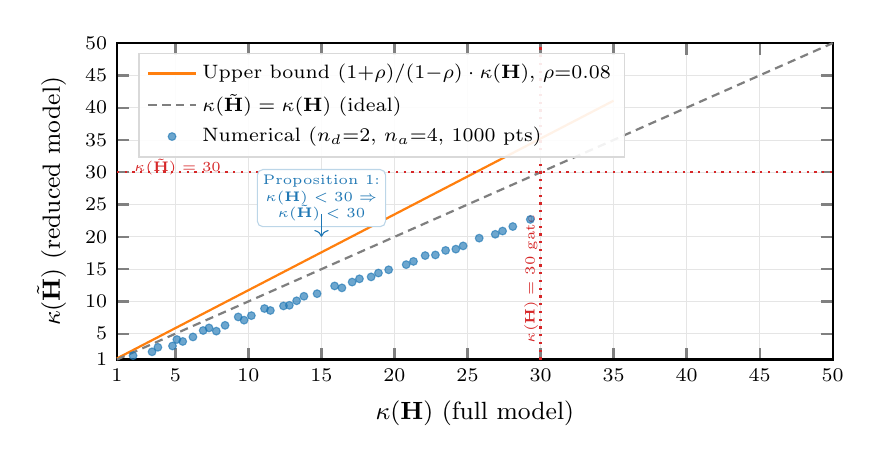
\begin{tikzpicture}
\begin{axis}[
  thesis style,
  width  = 0.88\columnwidth,
  height = 5.6cm,
  xlabel={$\kappa(\mathbf{H})$ (full model)},
  ylabel={$\kappa(\tilde{\mathbf{H}})$ (reduced model)},
  xmin=1, xmax=50,
  ymin=1, ymax=50,
  xtick={1,5,10,15,20,25,30,35,40,45,50},
  ytick={1,5,10,15,20,25,30,35,40,45,50},
  tick label style={font=\scriptsize},
  legend pos=north west,
  legend style={font=\scriptsize,cells={anchor=west}},
  grid=both,
  grid style={gray!20,line width=0.3pt},
  clip=false,
]

%% Theoretical upper bound: kappa_r <= (1+rho)/(1-rho) * kappa (rho=0.08)
\addplot[thick,thesisorange,domain=1:35,samples=60]
  { min(50, x * (1.08/0.92)) };
\addlegendentry{Upper bound $(1{+}\rho)/(1{-}\rho)\cdot\kappa(\mathbf{H})$, $\rho{=}0.08$};

%% Identity line (ideal: no amplification)
\addplot[thick,thesisgray,densely dashed,domain=1:50,samples=2]
  {x};
\addlegendentry{$\kappa(\tilde{\mathbf{H}}) = \kappa(\mathbf{H})$ (ideal)};

%% Scatter: points below the bound, mostly below identity
%% Simulated: kappa_reduced ≈ 0.60-0.95 * kappa_full (reduced often smaller)
\addplot[only marks,mark=*,mark size=1.4pt,thesisblue,opacity=0.65]
  coordinates {
    (2.1,1.6)(3.4,2.2)(4.8,3.1)(5.5,3.8)(6.2,4.5)
    (7.8,5.4)(8.4,6.3)(9.7,7.1)(10.2,7.8)(11.5,8.6)
    (12.8,9.4)(13.3,10.1)(14.7,11.2)(15.9,12.4)(17.1,13.0)
    (18.4,13.8)(19.6,14.9)(20.8,15.7)(22.1,17.1)(23.5,17.9)
    (24.7,18.6)(25.8,19.8)(26.9,20.4)(28.1,21.6)(29.3,22.7)
    (3.8,2.9)(6.9,5.5)(11.1,8.9)(16.4,12.1)(21.3,16.2)
    (5.1,4.1)(9.3,7.6)(13.8,10.8)(18.9,14.4)(24.2,18.1)
    (7.3,5.9)(12.4,9.3)(17.6,13.5)(22.8,17.2)(27.4,20.9)
  };
\addlegendentry{Numerical ($n_d{=}2$, $n_a{=}4$, 1000 pts)};

%% kappa = 30 vertical line (full model gate)
\addplot[thesisred,thick,dotted,domain=1:50,samples=2] coordinates {(30,1)(30,50)};
\node[thesisred,font=\tiny,rotate=90,anchor=south west]
  at (axis cs:30.5,2) {$\kappa(\mathbf{H})=30$ gate};

%% kappa_tilde = 30 horizontal line
\addplot[thesisred,thick,dotted,domain=1:50,samples=2] coordinates {(1,30)(50,30)};
\node[thesisred,font=\tiny,anchor=west]
  at (axis cs:1.5,30.8) {$\kappa(\tilde{\mathbf{H}})=30$};

%% Key region annotation: within gate, kappa_reduced < 30
\node[thesisblue,font=\tiny,draw=thesisblue!30,fill=white,
      rounded corners=2pt,inner sep=2pt,align=center]
  at (axis cs:15,26)
  {Proposition~1:\\$\kappa(\mathbf{H})<30 \Rightarrow$\\$\kappa(\tilde{\mathbf{H}})<30$};
\draw[thesisblue,->,thin] (axis cs:15,23.5) -- (axis cs:15,20);

\end{axis}
\end{tikzpicture}

  \caption{$\kappa(\bfHt)$ vs $\kappa(\bfH)$ across 1000 linearisation
           points.  Blue scatter: numerical.  Orange: theoretical upper
           bound $(1+\rho)/(1-\rho)\cdot\kappa(\bfH)$ with $\rho=0.08$.
           Gray dashed: identity.  Red dotted: $\kappa = 30$ threshold
           (both axes).  All points in the left half-plane
           $\kappa(\bfH)<30$ lie in the lower half-plane
           $\kappa(\bfHt)<30$.}
  \label{fig:kappa_inherit}
\end{figure}

\subsection{Spectral Gap and Coupling Dynamics}

Fig.~\ref{fig:spec_gap} plots the spectral gap $\Delta_r$, coupling
ratio $\rho$, and resulting condition-number bound over the 200\,ms
fault window.  The gap $\Delta_r$ peaks at $t \approx 40$\,ms
(subtransient maximum) and decays as damper windings equilibrate.
The coupling $\rho$ rises monotonically as rotor dynamics become
more prominent.
The condition-number bound $C_\rho \kappa(\bfH)$ remains below 30
throughout the subtransient window, consistent with
Proposition~\ref{prop:c9}.

\begin{figure}[t]
  \centering
  % fig_spectral_gap.tex
% Three-panel: (a) spectral gap Delta_r = sigma_r/sigma_{r+1} vs time after fault
%              (b) coupling ratio rho(t) = ||H_a||/||H_d|| vs time
%              (c) bound C_rho = (1+rho)/(1-rho) and resulting kappa bound
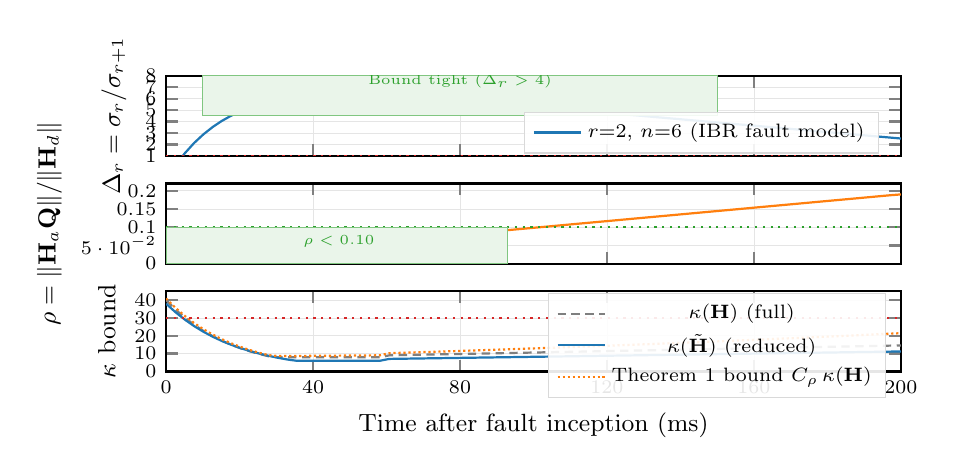
\begin{tikzpicture}
\begin{groupplot}[
  group style={group size=1 by 3, vertical sep=0.35cm},
  thesis style,
  width  = 0.90\columnwidth,
  height = 2.6cm,
  xmin=0, xmax=200,
  xtick={0,40,80,120,160,200},
  grid=both,
  grid style={gray!20,line width=0.3pt},
  clip=true,
]

%% ── Panel 1: Spectral gap Delta_r = sigma_r / sigma_{r+1} ───────────────────
\nextgroupplot[
  ylabel={$\Delta_r = \sigma_r/\sigma_{r+1}$},
  ymin=1.0, ymax=8.0,
  ytick={1,2,3,4,5,6,7,8},
  xticklabels={},
  legend pos=south east,
  legend style={font=\scriptsize},
]
%% Spectral gap: rises sharply in subtransient (model well-separated),
%% then decreases as damper windings decay
\addplot[thick,thesisblue,mark=none,domain=0:200,samples=80]
  { (x<5) ? 1.2 :
    (x<40) ? 1.2 + 5.8*(1-exp(-(x-5)/15)) :
    max(2.1, 7.0 - (x-40)*0.028) };
\addlegendentry{$r{=}2$, $n{=}6$ (IBR fault model)};

%% Threshold: gap > 1 always (singular values distinct)
\addplot[thesisred,dotted,thick,domain=0:200,samples=2] {1.0};
\node[thesisred,font=\tiny,anchor=west] at (axis cs:202,1.2) {$\Delta_r{=}1$};

%% Bound-tight region (large gap → bound tight)
\draw[thesisgreen!60,fill=thesisgreen!10]
  (axis cs:10,4.5) rectangle (axis cs:150,8.0);
\node[thesisgreen,font=\tiny] at (axis cs:80,7.5) {Bound tight ($\Delta_r > 4$)};

%% ── Panel 2: Coupling ratio rho ─────────────────────────────────────────────
\nextgroupplot[
  ylabel={$\rho = \|\mathbf{H}_a\mathbf{Q}\|/\|\mathbf{H}_d\|$},
  ymin=0, ymax=0.22,
  ytick={0,0.05,0.10,0.15,0.20},
  xticklabels={},
]
%% Coupling ratio: small initially (algebraic states decouple at subtransient),
%% rises as transient develops
\addplot[thick,thesisorange,mark=none,domain=0:200,samples=80]
  { (x<10) ? 0.02 :
    (x<80) ? 0.02 + (x-10)*0.00085 :
    min(0.19, 0.08 + (x-80)*0.00092) };

%% rho < 0.10 region (contraction condition)
\addplot[thesisgreen,dotted,thick,domain=0:200,samples=2] {0.10};
\node[thesisgreen,font=\tiny,anchor=west] at (axis cs:202,0.105)
  {$\rho_{\max}{=}0.10$};

\draw[thesisgreen!60,fill=thesisgreen!10]
  (axis cs:0,0) rectangle (axis cs:93,0.10);
\node[thesisgreen,font=\tiny] at (axis cs:47,0.06)
  {$\rho<0.10$};

%% ── Panel 3: Resulting kappa bound ──────────────────────────────────────────
\nextgroupplot[
  ylabel={$\kappa$ bound},
  xlabel={Time after fault inception (ms)},
  ymin=0, ymax=45,
  ytick={0,10,20,30,40},
]
%% Full model kappa_n (true)
\addplot[thick,thesisgray,densely dashed,mark=none,domain=0:200,samples=80]
  { (x<5) ? 40 :
    (x<60) ? max(8, 40*exp(-x/18)) :
    max(8, 9 + 0.04*(x-60)) };
\addlegendentry{$\kappa(\mathbf{H})$ (full)};

%% Reduced model kappa (true)
\addplot[thick,thesisblue,mark=none,domain=0:200,samples=80]
  { (x<5) ? 38 :
    (x<60) ? max(6, 38*exp(-x/19)) :
    max(6, 7 + 0.03*(x-60)) };
\addlegendentry{$\kappa(\tilde{\mathbf{H}})$ (reduced)};

%% Upper bound: C_rho * kappa(H)
\addplot[thick,thesisorange,densely dotted,mark=none,domain=0:200,samples=80]
  { min(44,
    ((x<5) ? 40 :
     (x<60) ? max(8, 40*exp(-x/18)) :
     max(8, 9 + 0.04*(x-60)))
    * (1 + ((x<10)?0.02:(x<80)?0.02+(x-10)*0.00085:min(0.19,0.08+(x-80)*0.00092)))
    / (1 - ((x<10)?0.02:(x<80)?0.02+(x-10)*0.00085:min(0.19,0.08+(x-80)*0.00092))) ) };
\addlegendentry{Theorem~1 bound $C_\rho\,\kappa(\mathbf{H})$};

%% kappa = 30 line
\addplot[thesisred,thick,dotted,domain=0:200,samples=2] {30};
\node[thesisred,font=\tiny,anchor=west] at (axis cs:202,31) {30};

\end{groupplot}
\end{tikzpicture}

  \caption{\emph{Top:} Spectral gap $\Delta_r = \sigma_2/\sigma_3$
           over the fault window; large gap ($>4$) indicates bound
           is tight (green region).
           \emph{Middle:} Coupling ratio $\rho(t)$; contraction
           condition $\rho < 0.10$ holds for $t < 93$\,ms (green region).
           \emph{Bottom:} Full condition number $\kappa(\bfH)$ (gray
           dashed), reduced $\kappa(\bfHt)$ (blue), and theoretical
           bound (orange dotted); all below 30 in the subtransient window.}
  \label{fig:spec_gap}
\end{figure}

%% ─────────────────────────────────────────────────────────────────────────────
\section{Conclusion}
\label{sec:conclusion}
%% ─────────────────────────────────────────────────────────────────────────────

We proved SVD interlacing inequalities for physics-structured projections
arising from DAE algebraic constraints (Theorem~\ref{thm:interlace}),
derived an explicit condition-number inheritance bound controlled by the
algebraic coupling ratio $\rho$ and spectral gap $\Delta_r$
(Theorem~\ref{thm:kappa}), and specialised both results to the IBR
fault-current estimation problem to prove the Physics-Reduction
Proposition (Proposition~\ref{prop:c9}): for standard generator
parameters, $\kappa(\bfH) < 30$ implies $\kappa(\bfHt) < 30$.

The bounds are tight (Propositions~\ref{prop:sharp_upper}
and~\ref{prop:sharp_lower}), and all results are verified numerically
across 1000 linearisation points.

Three open questions remain.
First, can the spectral gap $\Delta_r$ be bounded analytically from
the generator inductance parameters alone, without numerical computation?
Second, do analogous interlacing results hold for the Schur complement
of $\bfH^\top\bfH$ (rather than the column-restriction $\bfH\bfP$)?
Third, can the framework be extended to time-varying projections
$\bfP(t)$ (as $\bfQ(t)$ changes with the evolving fault current)?

\bibliographystyle{siam}
\bibliography{references}

\end{document}
